\documentclass[11pt]{article}
\usepackage[letterpaper,margin=0.9in]{geometry}
\usepackage[T1]{fontenc}
\usepackage{lmodern,microtype}
\usepackage{amsmath,amssymb,amsthm,mathtools}
\usepackage{graphicx,booktabs,array,tabularx,longtable}
\usepackage{enumitem,float,placeins}
\usepackage{caption}
\usepackage[hidelinks]{hyperref}
\hypersetup{pdftitle={Fixed-Budget Stop Design on Circular Routes},pdfauthor={Jiayu Ellie Su},pdfsubject={Continuum optimization, discrete stop placement, and observational timing calibration}}
\usepackage{fancyhdr}
\usepackage{url}
\setlength{\parindent}{0pt}
\setlength{\parskip}{5pt}
\setlength{\emergencystretch}{2em}
\setlist{nosep,leftmargin=*}
\captionsetup{font=small,labelfont=bf}
\pagestyle{fancy}\fancyhf{}
\fancyhead[L]{\small Fixed-budget stop design on circular routes}
\fancyhead[R]{\small Su}
\fancyfoot[C]{\thepage}
\setlength{\headheight}{14pt}
\newtheorem{theorem}{Theorem}[section]
\newtheorem{proposition}[theorem]{Proposition}
\newtheorem{corollary}[theorem]{Corollary}
\newtheorem{lemma}[theorem]{Lemma}
\theoremstyle{remark}\newtheorem{remark}[theorem]{Remark}
\newcommand{\C}{\mathcal C}
\newcommand{\Sset}{\mathcal S_N}
\newcommand{\E}{\mathbb E}
\newcommand{\ind}{\mathbf 1}
\newcommand{\osc}{\operatorname{osc}}
\newcommand{\clip}{\operatorname{clip}}
\title{\LARGE\bfseries Fixed-Budget Stop Design on Circular Routes\\[5pt]}
\author{Jiayu Ellie Su}
\date{}
\begin{document}
\maketitle
\begin{abstract}
Bus-stop design balances passenger access against delays imposed on through-riders, yet a continuous optimal density must ultimately be translated into feasible stop locations. This paper develops a fixed-budget formulation for heterogeneous circular routes, deriving the unique finite-cell solution $n_{N,i}^*=\sqrt{A_i/(B_i+\lambda)}$ and an exact identity for the cost of deviations from that solution. A constrained finite-site model is paired with a door-to-door evaluator that reassigns boarding and alighting stops, travel direction, and walk-only alternatives. Across 48 synthetic configurations and 720 training fits, the mean population excess cost of fixed-budget density projection falls from 14.23 seconds per trip using a single quantile phase to 1.64 seconds with phase selection and 0.60 seconds after two-stop-exchange refinement. A matched random-start search attains 0.61 seconds, indicating that discrete refinement explains much of the final improvement. In a separate chronological analysis of published shuttle observations, location-specific travel-time estimates fitted to October 2018 measurements reduce January 2019 mean absolute prediction error from 29.56 to 14.04 seconds across 90 interstop observations; location-specific stopped-duration estimates show no corresponding gain. The analysis identifies the roles of rounding, passenger reassignment, demand sampling, and component-level calibration in translating interpretable continuum models into discrete transit designs.
\end{abstract}
\smallskip
\textbf{Keywords:} bus-stop location; continuum approximation; fixed budget; discrete optimization; passenger assignment; reproducible benchmark.

\section{Introduction}
Bus-stop location determines both how far travelers walk and how much time they spend on a vehicle. Adding stops improves access to origins and destinations but increases delay for through-passengers. Continuum models capture this tradeoff through a spatial stop-density function. Transit planning, however, requires a finite set of locations subject to spacing, coverage, and siting constraints. The translation from a density to those locations introduces design choices that are absent from the continuous solution, while the resulting stop pattern can change passengers' boarding points, travel direction, and decision to ride.

This paper examines the relationship between the continuous design rule and the finite passenger-choice problem on circular routes. The analysis separates three stages: optimization of a fixed-budget density, conversion to feasible candidate sites, and evaluation after passenger reassignment. Keeping these stages distinct makes it possible to measure where approximation error enters and which computational refinements address it.

The theoretical analysis gives the unique fixed-budget solution for a finite spatial partition, an exact excess-cost identity, and bounds relevant to constrained density design and small movements of selected stops. The computational analysis compares density projection, phase selection, mixed-integer surrogate optimization, and local discrete search against exhaustive optima on a common feasible set. A chronological analysis of published loop-service measurements then evaluates the transfer of spatial travel-time and stopped-duration estimates across observation periods. Together, the mathematical, computational, and observational components characterize different sources of error in a practical stop-design workflow.

\subsection{Relationship to prior work}
Continuum formulations of stop spacing date to Wirasinghe and Ghoneim \cite{wirasinghe}; subsequent work has addressed heterogeneous transit demand and network structure \cite{ouyang}. Candidate-site optimization with access and through-passenger costs is developed by Furth and Rahbee \cite{furth}, while Mekuria, Furth, and Melachrinoudis \cite{mekuria} incorporate walking on a street network. Luo et al.\ \cite{luo} combine continuum approximations with constrained discrete optimization. Pandey and Lehe \cite{pandey} investigate heterogeneous trip lengths, demand response, and headway interactions.

The present study focuses on a fixed stop budget and explicit direction-specific operations on a circular route, with separate frozen-flow and reassignment-aware objectives. Its primary contribution is a controlled assessment of continuum-to-discrete performance under identical physical constraints, together with a temporally separated test of publicly reported timing measurements. The fixed-budget square-root rule provides the analytical benchmark; the finite-site experiments show how its performance depends on rounding and subsequent search.

\section{Continuum model and directional service}\label{sec:model}
\subsection{Geometry, demand, and operating assumptions}
Let $\C=[0,1)$ be a normalized circle. Demand is a nonnegative density $g(x,y)$ with $\int_{\C^2}g=1$; the corresponding origin and destination marginals are $f_O$ and $f_D$. Walking cost is $w(u)>0$ minutes per unit arc. The decision variable $n(u)\geq0$ is stop density, and $\int_\C n=N$ is the stop budget when imposed. A stop position represents a paired location in a two-direction model; individual curb-side infrastructure counts are not modeled separately.

For each offered direction $D$, let $k_D>0$ be its fleet, $b_D(u)>0$ its in-motion minutes per unit arc, and $\mu_D(u)>0$ the mean delay contributed by a selected stop. Let $A_D(x,y)$ be the directed open arc from $x$ to $y$. A fixed routing kernel satisfies $\sum_D\pi_D(x,y)=1$. Define
\begin{align}
\alpha_D&=\int_{\C^2}g(x,y)\pi_D(x,y)\,dx\,dy,\\
q_D(u)&=\int_{\C^2}g(x,y)\pi_D(x,y)\ind\{u\in A_D(x,y)\}\,dx\,dy,\label{eq:q}\\
m_{0,D}&=\int_\C b_D(u)\,du,\,
L_D(n)=m_{0,D}+\int_\C\mu_D(u)n(u)\,du.
\end{align}
Here $q_D$ is the fraction of potential riders whose fixed path crosses a location in direction $D$, not the local boarding density.

The continuum approximation assumes all-stop service, regular headways, independent random arrivals within the chosen direction's headway, and locally slowly varying coefficients and density. Mean wait is $L_D/(2k_D)$. Stop delay is exogenous to local boarding demand, and control holding time is excluded from the baseline formulation.

\subsection{Access, waiting, and through-rider burden}
Locally even spacing gives expected distance $1/(4n)$ from an endpoint to its nearest stop. Thus the access-plus-egress contribution is approximated by $\int_\C A/n$, where
\begin{equation}
A(u)=\frac{w(u)}4\bigl(f_O(u)+f_D(u)\bigr).
\end{equation}
Waiting and in-vehicle stop delay give the local coefficient
\begin{equation}
B(u)=\sum_D\mu_D(u)\left(\frac{\alpha_D}{2k_D}+q_D(u)\right).\label{eq:B}
\end{equation}
The design-independent part is
\begin{equation}
C_\pi=\sum_D\int_{\C^2}g\pi_D\int_{A_D(x,y)}b_D(u)\,du\,dx\,dy
+\sum_D\frac{\alpha_Dm_{0,D}}{2k_D}.
\end{equation}
Consequently,
\begin{equation}
\E[T]\approx C_\pi+J[n],\,
J[n]=\int_\C\left(\frac{A(u)}{n(u)}+B(u)n(u)\right)\,du.\label{eq:J}
\end{equation}
The expression follows by averaging each stop's delay across riders whose fixed arc contains it and adding directional waiting costs. Optimizing $J$ preserves the local-access and fixed-routing assumptions used in its derivation.

With equal directional fleets $k/2$, common stop delay $\mu$, and $q=q_{\rm cw}+q_{\rm ccw}$, equation~\eqref{eq:B} reduces to $B=\mu(1/k+q)$. For one direction with $k_D$ buses it instead becomes $B=\mu(1/(2k_D)+q_D)$. Directional fleet accounting is therefore explicit in each operating configuration.

\subsection{Free budget and structural interpretation}
For $A,B>0$, pointwise minimization gives
\begin{equation}
n^*(u)=\sqrt{A(u)/B(u)},\,
J[n^*]=2\int_\C\sqrt{A(u)B(u)}\,du.\label{eq:free}
\end{equation}
The identity $A/z+Bz-2\sqrt{AB}=(\sqrt{Bz}-\sqrt{A/z})^2$ proves the result whenever the quantities are integrable. Higher access pressure increases density, while larger stop delay or through-flow decreases it. For $A=0$, the convention $A/0=0$ gives zero optimal density in the unconstrained formulation. Discrete accessibility constraints are treated separately.

For independent uniform origins and destinations, symmetric shortest-arc assignment, $w=M$, and $\mu=s$, the mean selected arc length is $1/4$ and $q(u)=1/4$. Therefore
\begin{equation}
N^*=\sqrt{\frac{M}{2s(1/k+1/4)}}.\label{eq:homogeneous}
\end{equation}
The conclusion uses independence of the origin and destination coordinates: uniform marginals with spatially dependent trip endpoints may produce different through-flow.

\section{A fixed stop budget}\label{sec:budget}
\subsection{Finite piecewise-constant solution}
Partition the circle into finitely many cells of widths $\Delta_i>0$, with $\sum_i\Delta_i=1$. Use constant coefficients $A_i>0$ and $B_i>0$ in each cell. This is both a discretization of the analysis and the formulation implemented in the experiments.

\begin{theorem}[Fixed-budget density]\label{thm:budget}
For $N>0$, the problem
\begin{equation}
\min_{n_i>0}\sum_i\Delta_i\left(\frac{A_i}{n_i}+B_i n_i\right),\,
\sum_i\Delta_i n_i=N\label{eq:finite}
\end{equation}
has a unique solution
\begin{equation}
n_{N,i}^*=\sqrt{\frac{A_i}{B_i+\lambda}},\,
\sum_i\Delta_i\sqrt{\frac{A_i}{B_i+\lambda}}=N,\,
\lambda>-\min_iB_i.\label{eq:fixed}
\end{equation}
\end{theorem}
\begin{proof}
The Lagrangian has derivatives $\Delta_i(-A_i/n_i^2+B_i+\lambda)$. Its stationary equation gives~\eqref{eq:fixed}. The mass on the left is continuous and strictly decreasing in $\lambda$. It tends to zero as $\lambda\to\infty$, and to infinity as $\lambda\downarrow-\min_iB_i$, because a minimizing cell has positive width and positive $A_i$. Hence exactly one multiplier exists. The Hessian of the objective is diagonal with entries $2\Delta_i A_i/n_i^3>0$, so the feasible stationary point is the unique global minimizer.
\end{proof}

The analogous continuum expression characterizes the minimizer whenever a multiplier exists and the relevant integrals are finite. For arbitrary measurable coefficients, the multiplier equation may have no solution for some budgets; the finite-cell formulation above provides the existence result used in the experiments.

The multiplier is positive when the budget is below the free stop mass, zero when the two agree, and negative when the budget is larger. Rescaling $n^*$ by a common constant generally does not reproduce~\eqref{eq:fixed}, because adding $\lambda$ changes relative spatial penalties. If $B$ is constant, however,
\begin{equation}
n_N^*(u)=N\frac{\sqrt{A(u)}}{\int_\C\sqrt{A(v)}\,dv},
\end{equation}
so rescaling is exact. With spatially constant stop delays and a fixed budget, the waiting contribution of stops is also constant across layouts. It cannot explain relocation gains in that special case.

\subsection{Excess cost and density bounds}
\begin{proposition}[Exact excess-cost identity]\label{prop:gap}
Let $n_N^*>0$ be an admissible interior solution with $A=(B+\lambda)(n_N^*)^2$. For every positive density $n$ with the same budget and finite costs,
\begin{equation}
J[n]-J[n_N^*]=\int_\C(B(u)+\lambda)\frac{(n(u)-n_N^*(u))^2}{n(u)}\,du.\label{eq:gap}
\end{equation}
The corresponding weighted-sum identity holds for~\eqref{eq:finite}.
\end{proposition}
\begin{proof}
Substitution into the difference of integrands gives
\begin{equation*}
(B+\lambda)\left(\frac{(n_N^*)^2}{n}+n-2n_N^*\right)-\lambda(n-n_N^*).
\end{equation*}
The last term integrates to zero by equal budgets. The bracket is $(n-n_N^*)^2/n$.
\end{proof}
The identity supplies an objective-gap diagnostic and a solver check. If $|n/n_N^*-1|\leq\varepsilon<1$, it implies
\begin{equation}
J[n]-J[n_N^*]\leq\frac{\varepsilon^2}{1-\varepsilon}\int_\C(B+\lambda)n_N^*\,du.
\end{equation}
The identity and bound quantify differences within the continuous objective $J$, rather than between discrete passenger-journey evaluations.

Positive lower and finite upper density bounds can be incorporated without a new multivariate optimization. For $0<\underline n_i\leq\overline n_i<\infty$ and a feasible budget, define
\begin{equation}
n_i(\lambda)=
\begin{cases}
\clip\left(\sqrt{A_i/(B_i+\lambda)},\underline n_i,\overline n_i\right),&B_i+\lambda>0,\\
\overline n_i,&B_i+\lambda\leq0.
\end{cases}\label{eq:bounded}
\end{equation}
A multiplier satisfying $\sum_i\Delta_i n_i(\lambda)=N$ produces the unique minimizing density. This follows by minimizing each strictly convex Lagrangian term over its interval; its mass is continuous and nonincreasing. The multiplier need not be unique when all cells are at bounds, even though the density is unique. The bounded solver is implemented alongside explicit physical spacing constraints on selected candidate sites.

\begin{remark}[Zero-demand cells under a hard budget]
A free-budget express gap is not a universal fixed-budget conclusion. For two cells of width $1/2$, let $A=(1,0)$, $B=(2,1)$, and $N=2$. The budget is $n_1+n_2=4$, and the objective reduces to $(1/n_1+n_1+4)/2$. Its optimum is $(n_1,n_2)=(1,3)$, assigning density to the zero-access cell. Thus a fixed stop budget can allocate stop density to zero-access cells. The computational experiments use smoothed positive access coefficients.
\end{remark}

\section{Feasible discrete stops and reassigned journeys}\label{sec:discrete}
\subsection{A frozen-flow finite-candidate model}
Let $s_1,\ldots,s_m$ be candidate sites, $x_j\in\{0,1\}$ indicate selection, and $z_{rj}$ assign a demand endpoint in zone $r$ to a selected site. Let $a_r$ be boarding-plus-alighting probability mass, so $\sum_r a_r=2$, and let $c_{rj}$ be along-loop walking time. Holding the original directional paths fixed defines
\begin{align}
\min_{x,z}\ G(x,z)&=C_\pi+\sum_r a_r\sum_j c_{rj}z_{rj}+\sum_j B(s_j)x_j,\label{eq:milp}\\
\sum_j x_j&=N, &\sum_j z_{rj}&=1, &0\leq z_{rj}&\leq x_j.\nonumber
\end{align}
For integral $x$, minimizing over continuous $z$ yields nearest-stop access exactly. Mandatory and forbidden candidates fix corresponding $x_j$. Pairwise exclusions prohibit selected sites closer than the minimum gap. Maximum gaps are enforced by requiring a selected site in the forward maximum-gap window after every candidate. A covering constraint requires at least one site within the maximum nearest-stop walk of each zone, including zones with zero sampled demand.

All methods use the same feasible set $\Sset$. The accompanying mixed-integer implementation uses SciPy's \texttt{milp} interface \cite{scipy}; its solutions are independently checked for feasibility. In the small stress tests, direct enumeration of $G$ over $\Sset$ supplies the same exact finite comparator. Optimality certificates apply to the finite surrogate $G$; passenger reallocation is evaluated through $F$ below.

\subsection{A distinct passenger-choice objective}\label{sec:reassign}
For a selected stop set $S$, let $a,b\in S$ be distinct boarding and alighting stops. Directional ride time is
\begin{equation}
r_D(a,b;S)=\int_{A_D(a,b)}b_D(u)\,du
+\sum_{j\in S\cap A_D(a,b)}\mu_D(s_j)
+\frac{\mu_D(a)+\mu_D(b)}2.\label{eq:ride}
\end{equation}
Each selected journey assigns half of the endpoint dwell to boarding and alighting, with full dwell at intervening stops. With along-loop walking cost $c(x,a)$ and direct-walk time $c(x,y)$, define
\begin{align}
t_S(x,y)=\min\Bigl\{c(x,y),\ 
\min_{D,\,a\ne b\in S}\bigl[c(x,a)+c(y,b)+r_D(a,b;S)+L_D(S)/(2k_D)\bigr]\Bigr\},\label{eq:journey}\\
F_p(S)=\sum_{r,t}p_{rt}\,t_S(u_r,u_t).\label{eq:F}
\end{align}
Potential trips are retained when a traveler walks instead of riding, so $F$ measures expected time per potential trip. Direction choice is based on expected cost before vehicle arrival. Transfers and changes in total trip generation are outside this assignment model.

Unlike $G$, the objective $F$ recalculates ride distance, dwell exposure, direction shares, and the walk-only alternative for each layout. The difference $F-G$ therefore measures approximation error between the two model formulations. The nearest-stop constraint enforces physical coverage, independently of the access path selected by a traveler in~\eqref{eq:journey}.

The evaluator accommodates clockwise-only operation and unequal fleets in the two directions. The computational configurations use a shared circular geometry and a common set of candidate stop positions.

\subsection{Two error bounds with different meanings}
\begin{proposition}[Transfer from a surrogate]\label{prop:transfer}
On a nonempty finite feasible set, define $e(S)=F(S)-G(S)$. Then every $S\in\Sset$ satisfies
\begin{equation}
F(S)-\min_{T\in\Sset}F(T)
\leq G(S)-\min_{T\in\Sset}G(T)
+\underbrace{\max_T e(T)-\min_T e(T)}_{\osc_{\Sset}(e)}.\label{eq:transfer}
\end{equation}
\end{proposition}
\begin{proof}
Let $T_F$ minimize $F$. Then
$F(S)-F(T_F)=G(S)-G(T_F)+e(S)-e(T_F)$.
Use $G(T_F)\geq\min_TG(T)$ and bound the last difference by the oscillation.
\end{proof}
The bound decomposes discrete surrogate suboptimality and model-transfer error. Both terms can be evaluated for the small instances enumerated here; the discrepancy term can be conservative.

A different bound concerns movement of already labeled stops rather than changing objectives.
\begin{lemma}[Order-preserving stop displacement]\label{lem:snap}
Suppose two $N$-stop layouts $S,T$ have cyclically ordered, consistently lifted labels with $|s_j-t_j|\leq\delta$, and no change in cyclic order. Assume constant walking rate $W$, bounded in-motion rates $b_D\leq\overline b_D$, and Lipschitz stop delays with constants $K_D$. For the evaluator~\eqref{eq:journey},
\begin{equation}
\sup_{x,y}|t_S(x,y)-t_T(x,y)|
\leq\delta\max_D\left[2W+2\overline b_D+
\left(N-1+\frac{N}{2k_D}\right)K_D\right].\label{eq:snap}
\end{equation}
The same bound holds for $|F_p(S)-F_p(T)|$ under any common OD distribution.
\end{lemma}
\begin{proof}
Match a bus alternative to the same boarding label, alighting label, and direction in the other layout. Access and egress change by at most $2W\delta$. The two arc endpoints change the motion integral by at most $2\overline b_D\delta$. Cyclic order preserves the set of intervening labels. Their full dwell weights and the two half-endpoint weights sum to at most $N-1$, giving $(N-1)K_D\delta$. Cycle time changes by at most $NK_D\delta$, and hence wait by at most $NK_D\delta/(2k_D)$. Each matched alternative has this bound. Taking minima over matched alternatives and the common unchanged walking option preserves it. Averaging preserves it as well.
\end{proof}
The argument permits changes in the optimal passenger choice while preserving the cyclic correspondence of stops. Its hypotheses delimit the stability guarantee to small, order-preserving relocations with regular coefficients.

\section{From a density to a tested layout}\label{sec:algorithms}
\subsection{Projection and phase selection}
For a budget-normalized density define $H(u)=N^{-1}\int_0^u n(v)\,dv$. With phase $\theta\in[0,1)$, target sites are
\begin{equation}
v_j(\theta)=H^{-1}\left(\frac{j+\theta}{N}\right),\, j=0,\ldots,N-1.\label{eq:quantile}
\end{equation}
The phase controls the alignment of the target pattern with mandatory, prohibited, and other permissible sites. It is treated as a discrete design parameter during conversion from density to stops.

Each target set is projected by minimizing total circular matching distance over feasible $N$-site subsets and one-to-one target-site assignments. The experiments enumerate feasible subsets and solve the small assignment problem exactly for each. This agrees with the original matching MILP in independent tests. Ties use the lexicographically first feasible layout.

The phase-aware method uses $\theta=0,1/16,\ldots,15/16$. Repeated projected layouts are deduplicated, and a layout is selected by either $G$ or training-sample $F$. A uniform-density phase search provides a comparison for the effect of the heterogeneous density profile.

\subsection{Search and exact comparators}
A one-stop-exchange neighborhood replaces at most one selected candidate while retaining feasibility; a two-stop-exchange neighborhood replaces at most two. Best-improvement descent accepts strictly lower training cost until reaching a neighborhood-local optimum.

Original starting layouts are the reference, the single-phase free-density and fixed-budget projections, the access-only optimum, and the frozen-flow optimum. Phase-enhanced starts also include the best fixed-density and uniform-density phase designs. Two-stop search begins from these starts and their one-stop-descent endpoints. A no-density-start control keeps only the reference, access-only, frozen-flow, and uniform-phase starts. A further control adds randomly sampled feasible starts until its number of unique initial starts matches the density-enhanced method; its seed depends only on training counts. The matched-start comparison holds the number of unique initial solutions fixed; objective evaluations along subsequent search trajectories may differ.

Finally, exhaustive enumeration minimizes $F$ over the entire finite feasible set, providing a global comparator for the small instances. All designs use training data for selection; population and held-out costs are reserved for evaluation. The implementation precomputes costs and neighborhoods and limits enumeration to at most 100,000 candidate subsets.

\section{Computational experiments}\label{sec:experiment}
\subsection{Common geometry and operational parameters}
The experiment has 24 equally spaced candidates $s_j=j/24$, 32 demand zones $u_r=(r+1/2)/32$, and $N=8$ selected positions. Candidates 0 and 12 are mandatory; 5 and 17 are forbidden. The reference is $(0,3,6,9,12,15,18,21)$. Minimum gap is 0.055 of a loop. Maximum gap is either 0.23 or 0.18, and maximum nearest-stop walking time is 12 minutes. These are experimental siting constraints. For a 6 km loop they correspond to a 330 m minimum gap and maximum gaps of 1,380 m and 1,080 m.

Walking around the complete loop takes 90 minutes; in-motion circulation takes 18 minutes. Let $d_\C$ be circular distance and $h(u;c,\sigma)=\exp[-d_\C(u,c)^2/(2\sigma^2)]$. Heterogeneous stop delays are
\begin{equation}
\mu(u)=0.18+0.55h(u;0.39,0.08)+0.23h(u;0.78,0.10)\,\text{minutes}.\label{eq:dwell}
\end{equation}
At the candidate sites these range from 0.183 to 0.720 minutes. The constant-delay control uses their mean, 0.347944 minutes. Service is either symmetric with three buses per direction, clockwise-only with three buses, or unequal with four clockwise and two counterclockwise buses. The one-way configuration uses a smaller total fleet, so its results reflect both service direction and frequency.

There are 38,760 subsets satisfying the cardinality and mandatory/forbidden restrictions before gap and coverage filtering. The two maximum-gap regimes leave 508 and 243 feasible layouts, respectively. The corresponding one-stop-exchange graphs are connected.

\subsection{Demand families and train-test separation}
Four synthetic OD generators are used: uniform off-diagonal demand, short local trips with kernel $\exp(-d_\C/0.06)$, a two-hub mixture, and a commuter mixture with a concentrated destination. Exact formulas are in Appendix~\ref{app:demand} and the executable generator. Diagonal mass is removed before final normalization.

The main factorial design combines four demand families, two dwell patterns, three service patterns, and two gap regimes, giving 48 structural configurations. Each has five independently generated training-count samples of 3,000 trips and a separate 12,000-trip test sample, giving 240 fits. The same procedure at training sizes 300 and 30,000 gives another 480 fits. The documented seed sequence is shared across sample sizes to support controlled comparisons of sample-size sensitivity.

Density coefficients use a 128-bin circular histogram of endpoint mass, Gaussian smoothing with standard deviation two bins, and a 1\% uniform component. These regularization parameters are fixed across experiments. Frozen routing minimizes no-stop in-motion time, with equal splitting of ties. In the unequal-fleet case it deliberately ignores waiting when defining the exogenous kernel; the reassigned evaluator does not.

\subsection{Performance criteria}
For the known generating distribution $P$, the population oracle is
\begin{equation}
S_P^*\in\arg\min_{S\in\Sset}F_P(S).
\end{equation}
The principal metric is \emph{population excess cost}, or regret,
$60[F_P(\widehat S)-F_P(S_P^*)]$ seconds per potential trip. Since $P$ is known for the synthetic generators, the population expectation is computed exactly over the finite OD support. Training procedures do not use the population oracle when selecting designs.

Training excess cost compares a selected method with the exhaustive minimum of $F_{\widehat P}$. A method can have zero training excess cost and positive population excess cost. Conversely, a slightly suboptimal training method can outperform the training optimum on the population distribution by fitting sampling noise less closely.

An illustrative case uses seed 20261031, 3,000 training trips, and 12,000 held-out synthetic trips. A paired bootstrap resamples the held-out trips with the chosen layouts fixed. Across-configuration summaries characterize the specified factorial design and are reported descriptively.

\section{Results}\label{sec:results}
\subsection{Illustrative instance and phase sensitivity}
In the illustrative instance, the fixed-budget solution attains a continuous objective of 6.616867 minutes excluding the common constant, compared with 6.781400 for proportional rescaling of the free-budget density. The multiplier is 0.562606, and the identity~\eqref{eq:gap} agrees with the numerical objective difference to within $4\times10^{-16}$ minutes.

Projection at a fixed half-phase produces a layout 15.28 seconds per held-out trip slower than the reference. Across 16 phases, the same density yields ten distinct layouts. Selecting by reassigned training time identifies the exhaustive training optimum, $(0,2,4,8,12,14,16,20)$, which saves 10.20 seconds per held-out synthetic trip relative to the reference, or 1.39\% of its mean time. A paired bootstrap with 1,000 resamples gives a conditional 95\% percentile interval of 7.11 to 13.52 seconds for this difference.

Phase selection from a \emph{uniform} density also identifies the optimum in this instance. The comparison isolates the contribution of phase-aware discrete search from that of the heterogeneous density profile (Table~\ref{tab:case}).

\begin{table}[htbp]\centering\small
\caption{Illustrative synthetic instance. Savings are relative to the reference layout; the training gap is relative to the exhaustive reassignment optimum.}\label{tab:case}
\begin{tabular}{@{}p{3.23in}rrr@{}}\toprule
Method & Test mean & Saving & Train gap\\
 & (min) & (s/trip) & (s/trip)\\\midrule
% BEGIN GENERATED case
Reference & 12.2236 & 0.00 & 12.07 \\
Rescaled free density, one phase & 12.5286 & -18.30 & 28.96 \\
Fixed-budget density, one phase & 12.4783 & -15.28 & 29.87 \\
Exact frozen-flow design & 12.2236 & 0.00 & 12.07 \\
Fixed density, 16 phases & 12.0537 & 10.20 & 0.00 \\
Uniform density, 16 phases & 12.0537 & 10.20 & 0.00 \\
One-swap, original starts & 12.1363 & 5.24 & 4.41 \\
One-swap, phase starts & 12.0537 & 10.20 & 0.00 \\
Two-swap, phase starts & 12.0537 & 10.20 & 0.00 \\
Two-swap, no density starts & 12.0537 & 10.20 & 0.00 \\
Two-swap, matched random starts & 12.0537 & 10.20 & 0.00 \\
Exact training reassignment & 12.0537 & 10.20 & 0.00 \\
% END GENERATED case
\bottomrule\end{tabular}
\end{table}

\begin{figure}[htbp]\centering
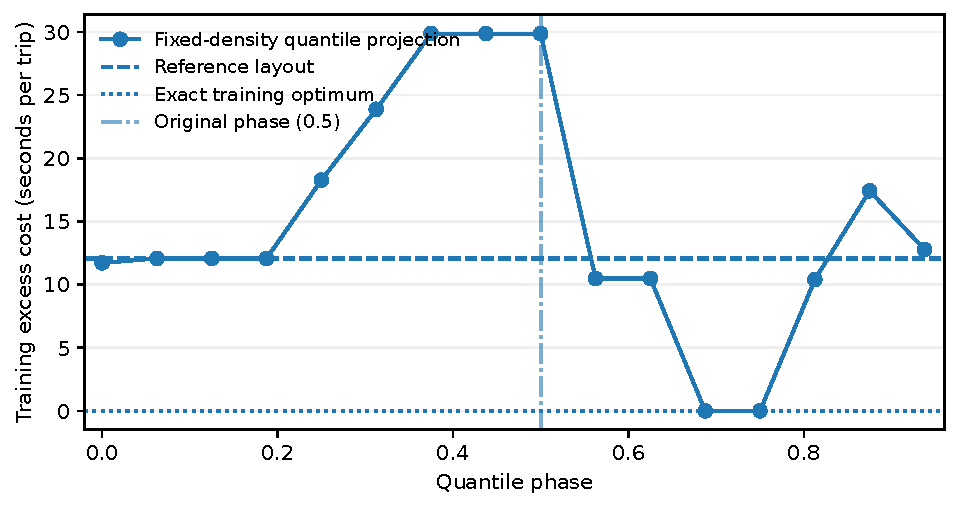
\includegraphics[width=.90\linewidth]{figures/phase_effect.pdf}
\caption{Phase sensitivity of fixed-budget density projection. The zero level is the exhaustive training optimum.}\label{fig:phase}
\end{figure}

The frozen-flow optimum is the reference layout, but its reassigned training gap is 12.07 seconds. The discrepancy oscillation in~\eqref{eq:transfer} is 44.15 seconds, giving a valid but loose bound. The Spearman correlation of frozen and reassigned costs over all 508 layouts is 0.925. High overall rank correlation therefore does not guarantee agreement about the best layout. Figure~\ref{fig:landscape} makes that distinction visible.

\begin{figure}[htbp]\centering
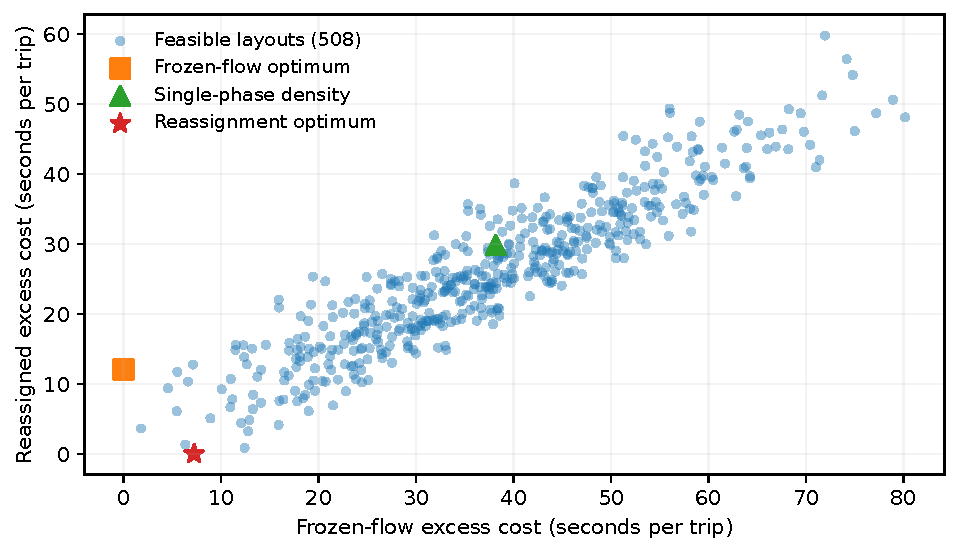
\includegraphics[width=.90\linewidth]{figures/surrogate_landscape.pdf}
\caption{All 508 feasible layouts in the detailed case. Both axes measure excess training cost relative to their own objective's minimum. The two minimizers differ even though the objectives are strongly rank-correlated.}\label{fig:landscape}
\end{figure}
\FloatBarrier

\subsection{The 48-configuration benchmark}
Table~\ref{tab:suite} summarizes the 240 fits at 3,000 training trips. Single-phase fixed-budget conversion incurs 14.23 seconds of mean population excess cost, compared with 13.38 seconds for the reference layout, and performs worse than the reference in 180 of 240 fits. Rescaled free-density projection also loses to the reference in 180 fits, although its aggregate mean excess cost is 12.63 seconds because it performs better in other configurations. These comparisons quantify losses arising from the discrete projection stage.

Phase selection with reassigned training cost reduces the fixed-density mean error to 1.64 seconds. Selecting phases under the frozen objective instead gives 3.18 seconds, compared with 2.96 seconds for exhaustive frozen-flow optimization. These comparisons separate discretization from objective mismatch. Uniform-density phase search gives 3.63 seconds, so the heterogeneous density is informative at the phase-proposal stage in this particular factorial grid.

\begin{table}[htbp]\centering\small
\caption{Main synthetic benchmark: 48 configurations, five samples each, 3,000 training trips. Mean and 95th percentile are population excess costs. ``Exact fits'' counts equality, within $10^{-6}$ seconds, with the exhaustive training optimum.}\label{tab:suite}
\begin{tabular}{@{}p{3.25in}rrr@{}}\toprule
Method & Mean (s) & 95th (s) & Exact fits\\\midrule
% BEGIN GENERATED suite
Reference & 13.38 & 45.85 & 20/240 \\
Rescaled free density, one phase & 12.63 & 32.39 & 3/240 \\
Fixed-budget density, one phase & 14.23 & 31.53 & 3/240 \\
Exact frozen-flow design & 2.96 & 10.18 & 26/240 \\
Fixed density, 16 phases & 1.64 & 5.67 & 53/240 \\
Uniform density, 16 phases & 3.63 & 12.78 & 33/240 \\
One-swap, original starts & 1.08 & 4.50 & 139/240 \\
One-swap, phase starts & 0.79 & 3.02 & 159/240 \\
Two-swap, phase starts & 0.60 & 2.74 & 233/240 \\
Two-swap, no density starts & 0.59 & 2.74 & 212/240 \\
Two-swap, matched random starts & 0.61 & 2.74 & 235/240 \\
Exact training reassignment & 0.60 & 2.74 & 240/240 \\
% END GENERATED suite
\bottomrule\end{tabular}
\end{table}

With phase-selected starting layouts, one-stop exchange reduces mean population excess cost to 0.79 seconds and reaches the exact training optimum in 159 of 240 fits. Two-stop exchange reduces the mean excess cost to 0.60 seconds and reaches that optimum in 233 fits. Exhaustive enumeration supplies the global comparator in all 240 fits.

Control experiments separate the effects of starting layouts and discrete refinement. Two-stop search without density-based starts attains 0.59 seconds of mean population excess cost and 212 exact training optima. Matched random starts give 0.61 seconds and 235 optima. The close population results show that strong discrete search accounts for much of the final accuracy, while density-based phase selection is a useful way to propose initial layouts.

\begin{figure}[htbp]\centering
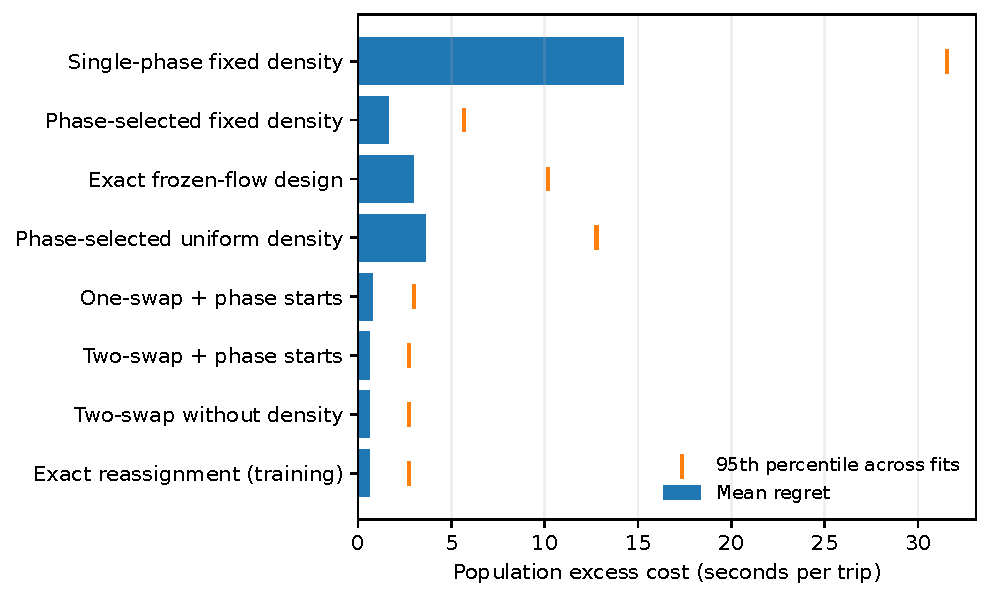
\includegraphics[width=.97\linewidth]{figures/benchmark_regret.pdf}
\caption{Population regret in the 240-fit synthetic benchmark. Horizontal bars show means; tick markers show empirical 95th percentiles across fits.}\label{fig:regret}
\end{figure}

Demand structure matters. Reference mean regret is 43.83 seconds in the commuter family but only 0.052 seconds in the short-local family. The reference is already nearly optimal for many short trips because walking competes effectively with the bus. Optimizing a noisy demand sample can then produce slight deterioration even when it minimizes training time exactly. Figure~\ref{fig:demand} displays the variation by demand family.

\begin{figure}[htbp]\centering
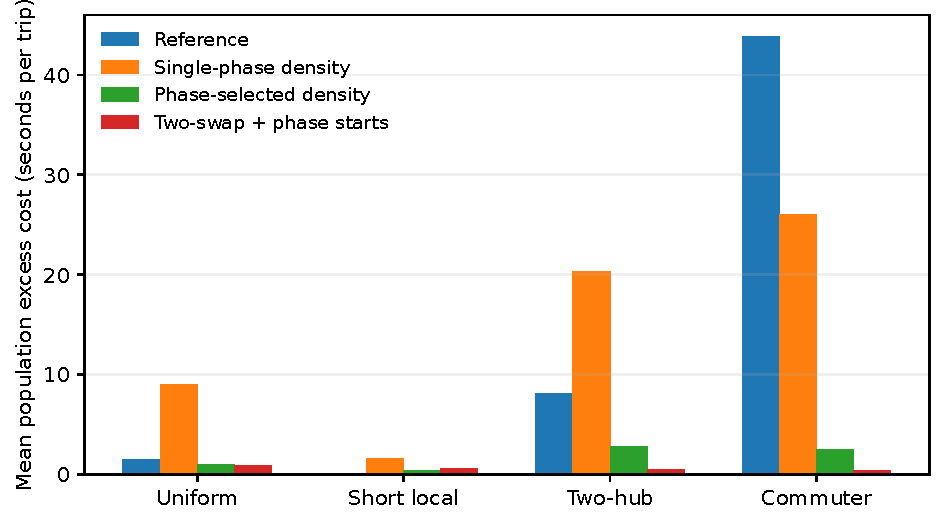
\includegraphics[width=.90\linewidth]{figures/demand_families.pdf}
\caption{Population regret by synthetic demand family, averaging over the other design factors and five training samples. The same algorithm can face a large opportunity in one family and almost none in another.}\label{fig:demand}
\end{figure}
\FloatBarrier

\subsection{Demand estimation can dominate search error}
Table~\ref{tab:sample} and Figure~\ref{fig:sample} distinguish optimization error from demand-estimation error. For exhaustive training optimization, mean population regret falls from 3.126 seconds with 300 trips to 0.601 with 3,000 and 0.088 with 30,000. The globally optimal training design nevertheless performs worse than the reference in 111, 64, and 27 of the respective 240 fits, reflecting sampling variation and differences in the gains available across demand patterns.

The two-stop method and matched random-start control show similar learning curves. A local-search layout can have lower population regret than the exhaustive training minimizer because the latter optimizes the sampled objective. This separates errors due to demand estimation from errors due to finite search.

\begin{table}[htbp]\centering\small
\caption{Mean population excess cost in seconds per trip. Each training size uses 240 fits over the same 48 structural configurations.}\label{tab:sample}
\begin{tabular}{@{}rrrrr@{}}\toprule
Training trips & Density + phases & Two-swap + phases & Matched random & Exact training\\\midrule
% BEGIN GENERATED sample
300 & 3.225 & 3.148 & 3.134 & 3.126\\
3,000 & 1.637 & 0.598 & 0.608 & 0.601\\
30,000 & 1.231 & 0.074 & 0.078 & 0.088\\
% END GENERATED sample
\bottomrule\end{tabular}
\end{table}
\begin{figure}[htbp]\centering
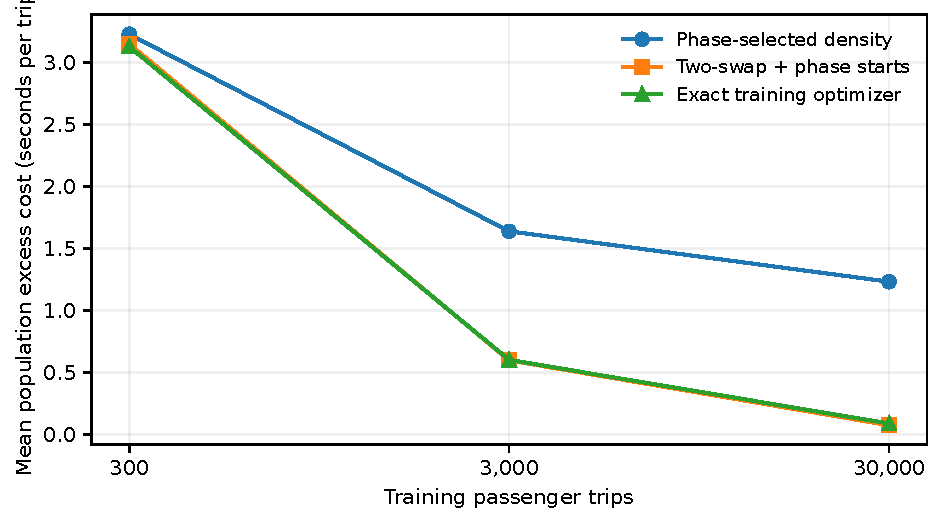
\includegraphics[width=.90\linewidth]{figures/sample_size.pdf}
\caption{Population excess cost by training-sample size, computed exactly under each synthetic OD distribution.}\label{fig:sample}
\end{figure}

\subsection{Parameter sensitivity and minimax regret}
For the detailed case, all feasible layouts are evaluated at walking-time multipliers $0.8,1,1.2$ and dwell multipliers $0.5,1,1.5$. Let $F_\omega$ denote a scenario's training objective. The finite scenario minimax-regret design minimizes
\begin{equation}
\max_{\omega}\left[F_\omega(S)-\min_{T\in\Sset}F_\omega(T)\right].\label{eq:robust}
\end{equation}
Its scenario set and all design selection use training data only. In this case the minimax and nominal exact designs coincide. Their worst training scenario regret is 3.20 seconds, and their held-out savings relative to the fixed reference range from 3.97 to 12.91 seconds. These nine scenarios characterize the parameter sensitivity of the illustrative finite instance.
\FloatBarrier

\section{Observational calibration on an existing loop route}\label{sec:observed}
\subsection{Source observations and temporal design}
The observational analysis uses published Orangeline measurements from Videa and Wang's Streamline study \cite{videa}. The source includes an April 2018 passenger origin--destination survey (Table~9, printed pages~32--33), interstop travel times (Table~16, page~55), and stopped durations (Table~17, page~56). The 19-by-19 survey matrix records 23 trips pooled across survey days. Timing observations provide a distinct dataset for the predictive analysis below.

The timing tables contain ten collection columns: five from October 2018 and five from January 7--11, 2019. October observations are used to fit location-specific and pooled predictors, and January observations are reserved for a chronological test. This design evaluates the portability of travel-time and stopped-duration estimates between collection periods.

Table entries were transcribed from the published report text and cross-checked across available hosted versions. The reported timing means and sample standard deviations agree with the transcription to within 0.002 seconds, consistent with rounding; survey row and column totals also reconcile. The complete tabulations and provenance checks accompany the code, with additional source details in Appendix~\ref{app:observed}.

\subsection{Cleaning, missingness, and chronological separation}
There are 85 numeric October travel times and 95 January travel times over 19 links. One link, numbered 12--13 in the source, has no October measurement. The primary comparison uses the 90 January observations on the 18 links with training support. A secondary comparison includes all 95 observations, assigning the unobserved-in-training link a training-pooled fallback. It never fits that link using January values.

The stopped-time table repeats identical October values in terminal rows 1 and 20 and records no January values in either. Both terminal rows are excluded from stopped-time fitting and scoring, avoiding duplicated terminal observations. The remaining 18 stop positions provide 37 numeric October durations and 31 January durations. Two January durations are at a stop with no October duration, leaving 29 observations on common support. Recorded stopped durations represent a sparse subset of stop events.

A dash is retained as missing, never as a zero. The source explains that travel-time omissions include recording errors, whereas stopped-time omissions can also mean that the bus did not stop \cite{videa}. Accordingly, the stopped-duration outcome is \emph{duration conditional on a recorded numeric entry}; it differs from the unconditional stop-delay coefficient $\mu_D$ of the all-stop design model.

Repeated October date labels are preserved as separate collection columns, not interpreted as distinct days. Table~16 labels its first column October~8, while Table~17 labels that column October~18. The month-based split is unaffected, but the mismatch precludes a verified run-by-run join. Travel and stopped durations are consequently analyzed separately. The survey and timing tables also have different stop-label sets, so their IDs are kept separate.

\subsection{Predictors, errors, and day-level uncertainty}
For location $\ell$, let $\mathcal O_\ell$ be its recorded October observations. The location-mean predictor is
\begin{equation}
\widehat t_\ell=\frac{1}{|\mathcal O_\ell|}\sum_{r\in\mathcal O_\ell}t_{\ell r}.
\end{equation}
The pooled-mean baseline averages all recorded training observations for the quantity being predicted. Median analogues provide two additional untuned baselines. An unseen location receives the corresponding pooled training statistic. All four prespecified predictors are fitted to October data and scored without refitting on January observations. The pooled travel-time baseline is a deliberately simple comparator that does not adjust for differences in link length.

Table~\ref{tab:observed} reports mean absolute error (MAE), root mean squared error (RMSE), and prediction-minus-observation bias. Travel and stopped-duration errors are reported separately because their support sets and outcome definitions differ.
\begin{table}[htbp]\centering\small
\caption{Chronological prediction errors on January 7--11, 2019 observations with October training support. Travel includes 90 link observations; stopped duration includes 29 numeric observations. Bias is prediction minus observation. All values are in seconds per observation.}\label{tab:observed}
\begin{tabular}{llrrrr}
\toprule
Quantity & Predictor & $n$ & MAE (s) & RMSE (s) & Bias (s)\\
\midrule
Travel & Pooled mean & 90 & 29.56 & 36.83 & 4.40\\
Travel & Pooled median & 90 & 28.93 & 36.57 & -0.14\\
Travel & Location mean & 90 & 14.04 & 18.32 & 3.83\\
Travel & Location median & 90 & 13.49 & 18.03 & 3.08\\
\midrule
Stopped & Pooled mean & 29 & 14.17 & 26.12 & -13.17\\
Stopped & Pooled median & 29 & 14.97 & 26.71 & -14.30\\
Stopped & Location mean & 29 & 14.66 & 25.69 & -13.28\\
Stopped & Location median & 29 & 15.80 & 26.57 & -14.39\\
\bottomrule
\end{tabular}

\end{table}

Location-mean travel prediction reduces MAE from 29.56 to 14.04 seconds and improves on the pooled mean on each held-out day. Location medians give MAE 13.49 seconds. With all 95 travel observations and the prescribed fallback, mean-predictor MAEs are 30.29 seconds pooled and 15.60 seconds location-specific. The improvement demonstrates the predictive value of link-specific timing estimates for these observations; unequal link lengths may explain part of the difference.

Stopped-duration prediction does not show the same benefit. On common support, pooled-mean MAE is 14.17 seconds and location-mean MAE is 14.66 seconds. Location-mean bias is $-13.28$ seconds, indicating substantial underprediction of the recorded January durations. On all 31 January stopped observations, the respective MAEs are 13.56 and 14.02 seconds. Thus spatial stratification improves interstop predictions in this dataset but not the sparse stopped-duration predictions.

Uncertainty is summarized at the held-out day level, not by treating all links as independent replications. Define daily gain $g_d=\mathrm{MAE}_{d,\mathrm{pooled}}-\mathrm{MAE}_{d,\mathrm{location}}$, with equal weight per day. Enumerating all $5^5=3{,}125$ ordered five-day bootstrap resamples gives a travel gain of 15.52 seconds and a 95\% percentile range of 13.41 to 17.86 seconds. For stopped duration, the day-weighted gain is $-0.72$ seconds with a range of $-1.94$ to 0.34 seconds. These intervals describe day-level resampling variation for five adjacent held-out dates, conditional on the October fits. Daily errors and predictions are provided in the repository.

\begin{figure}[htbp]\centering
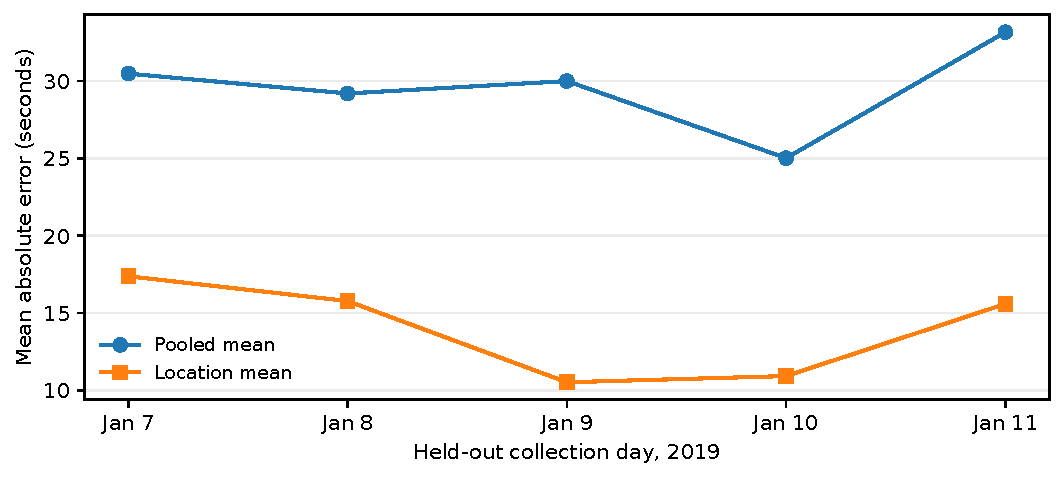
\includegraphics[width=.84\textwidth]{figures/observed_travel_daily.pdf}
\caption{Held-out interstop travel-time prediction error by January service day, using link-level predictors fitted in October.}\label{fig:observedtravel}
\end{figure}
\begin{figure}[htbp]\centering
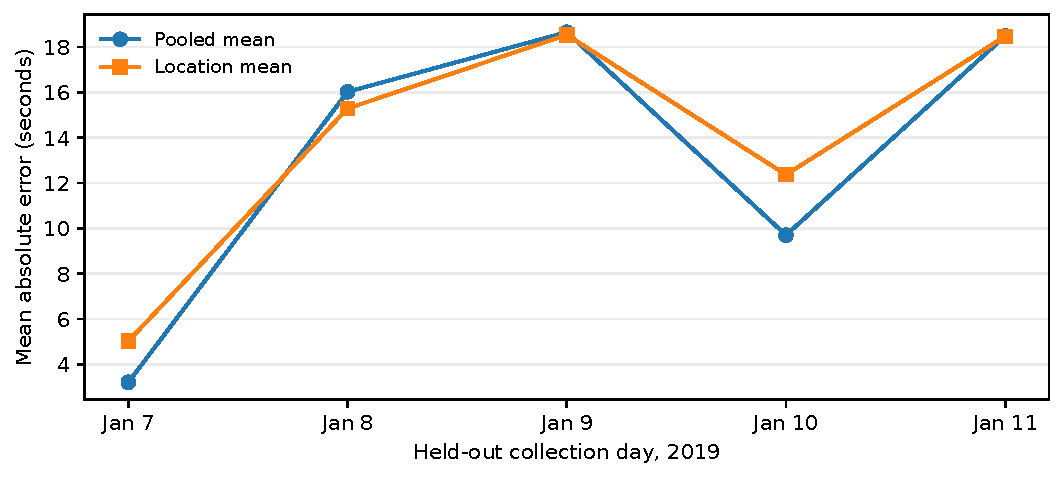
\includegraphics[width=.84\textwidth]{figures/observed_stopped_daily.pdf}
\caption{Held-out prediction error for recorded stopped duration on the common-support stop set.}\label{fig:observedstopped}
\end{figure}
\FloatBarrier

\subsection{Interpretation}
The chronological test measures prediction of timing components under the observed service configuration. Location-specific link means transfer better than pooled means across the two periods, whereas stopped-duration observations are too sparse to yield the same gain. These component estimates can inform subsequent service models, provided their definitions are retained: observed stopped duration conditional on a recorded event is not the additional delay caused by installing a stop.

The published April survey supplies pooled OD observations, not January day-specific demand, and the survey and timing tables have unmatched stop identifiers. A counterfactual stop-location comparison would additionally require a consistent origin--destination model, pedestrian-network access costs, candidate-site feasibility, and a calibrated relationship between demand and stopping delays. The findings here are therefore interpreted as temporal calibration of an existing service, separately from the synthetic evaluations of alternative stop layouts.

\section{Operational considerations}\label{sec:limits}
\subsection{Capacity and accessibility}
For a bus-rider arrival rate $\Lambda$, directional capacity $C_D$, and fixed-rider through-flow $q_D$, a necessary throughput condition is
\begin{equation}
\Lambda q_D(u)\leq\frac{k_D C_D}{L_D(n)}\quad\text{for almost every }u.\label{eq:capacity}
\end{equation}
The right-hand side is the seating flow provided by $k_D$ buses crossing the location once per cycle. For a layout evaluated under~\eqref{eq:journey}, through-flow and direction assignment must be recalculated for the selected passengers. The capacity condition is necessary rather than sufficient when loads and arrivals vary over time.

The computational candidate sets impose mandatory locations, minimum and maximum spacing, and coverage radii along the modeled loop. An operational candidate set would also encode curb geometry, accessible crossings, pedestrian routes, transfers, vehicle access, and other site-specific restrictions. Such details can alter both the feasible locations and the resulting travel-time objective.

\subsection{Headway variation and reliability}
The passenger evaluator uses stabilized directional headways. Under a stationary renewal model with independent random passenger arrivals and nonconstant headways $H$, the mean residual wait instead satisfies
\begin{equation}
\E[W]=\frac{\E[H^2]}{2\E[H]}.
\end{equation}
Thus the waiting component becomes sensitive to headway variability as well as mean frequency. The synthetic study evaluates deterministic expected journey times, and its cross-passenger dispersion describes heterogeneity in trips rather than stochastic service reliability. A route-specific reliability model would account for headways, vehicle movement, dwell, and control jointly.

\section{Discussion and conclusion}
The fixed-budget stop-density law provides an interpretable allocation of stop intensity between local access demand and through-passenger delay. Its multiplier enforces the prescribed total number of stops, while the exact objective-gap identity quantifies departures from the continuous optimum. The corresponding finite candidate-site problem adds physical constraints and changes the passenger-choice objective through boarding, alighting, directional assignment, and walking alternatives.

The computational results establish that these transitions have measurable consequences. A single quantile phase performs inconsistently even when the density satisfies the fixed-budget optimum. Searching over phases reduces mean population excess cost from 14.23 to 1.64 seconds per potential trip in the 3,000-trip synthetic benchmark. Two-stop-exchange refinement lowers it to 0.60 seconds and reaches the exact training optimum in 233 of 240 fits. The matched random-start control performs similarly, locating the principal gains in feasible discrete search rather than in one particular initialization. Across the three training sizes, the remaining population error decreases markedly as demand information improves, illustrating the separate roles of statistical estimation and optimization.

The observational analysis complements these design experiments with a temporally separated calibration test. On the published Orangeline measurements, location-specific interstop averages predict the later January collection substantially more accurately than an unstratified pooled mean. The stopped-duration measurements behave differently: location stratification offers no improvement on the sparse common-support sample. The two outcomes underscore the need to distinguish in-motion timing, stopping duration, and passenger assignment rather than treating them as a single calibrated coefficient.

The results support a practical modeling sequence: use the continuum solution to characterize spatial tradeoffs and generate candidate patterns; evaluate multiple projections under the actual feasible set; refine layouts with reassignment-aware objectives; and estimate timing and demand components from data with their definitions and uncertainties preserved. This sequence connects a transparent analytical design law to discrete optimization while clarifying which gains arise from rounding, search, and information quality. Observed timing calibration establishes predictive performance for existing service components; realized effects of stop changes remain a separate question for route-specific counterfactual evaluation or field implementation.

\section*{Data and code availability}
The accompanying repository contains the LaTeX manuscript, figure-generation scripts, candidate-site and assignment algorithms, complete synthetic count samples and outputs from 720 fits, transcriptions of published observations, fitted predictors, and chronological evaluation results. The computational test suite includes 29 tests. The synthetic and observational datasets are identified separately, and the provenance of the observational tabulations is documented in Appendix~\ref{app:observed}.


\appendix
\section{Synthetic OD distributions}\label{app:demand}
Let $\mathcal N(M)=M/\sum_{r,t}M_{rt}$, and write $d_{rt}=d_\C(u_r,u_t)$. Each expression below is evaluated on the 32 zones; after construction its diagonal is set to zero and it is normalized again. Uniform demand is $P=\mathcal N(\mathbf1\mathbf1^\top)$ before diagonal removal. Local demand is $P=\mathcal N(\exp(-d_{rt}/0.06))$.

For two-hub demand, define
\begin{align*}
a_r&=0.15+2.5h(u_r;0.13,0.065)+1.8h(u_r;0.59,0.075),\\
b_r&=0.15+2.2h(u_r;0.34,0.065)+1.7h(u_r;0.85,0.065),\\
P^{\rm pre}&=0.7\mathcal N(ab^\top)+0.3\mathcal N(\exp(-d_{rt}/0.12)).
\end{align*}
For commuter demand, define
\begin{align*}
a_r&=0.25+2h(u_r;0.18,0.08)+1.3h(u_r;0.78,0.06),\\
b_r&=0.03+3h(u_r;0.48,0.045),\\
P^{\rm pre}&=0.65\mathcal N(ab^\top)+0.25\mathcal N(ba^\top)
+0.10\mathcal N(\exp(-d_{rt}/0.10)).
\end{align*}
Training and test counts are multinomial draws from these distributions. The main detailed case uses seed 20261031. For the factorial suite, configurations follow the order encoded in \texttt{experiments.py}, and fit $j$ uses seed $730000+j$. The sequence is reused across training-sample sizes. All generated count arrays are provided with the repository.

\section{Observed-data provenance and reproduction}\label{app:observed}
The source study is Videa and Wang \cite{videa}. The analysis uses aggregate values from the published tables rather than the original raw-device recordings; no device identifiers are included. The transcriptions were checked against published text and tabular summaries, but the source page images were not independently inspected.

\texttt{data/observed/orange\_timing\_long.csv} retains all 390 table cells, including missing entries, the original date label, collection-column number, quantity, stop/link label, source table, and printed page. \texttt{orange\_survey\_od.csv} retains all 361 OD cells, not just the nonzero values. The survey total is 23 trips in 15 nonzero OD cells; both row and column margins agree exactly with the DOT and university PDF text. A structured extraction from one hosted version omits the origin-11, destination-6 entry, while two alternative versions show one trip in that cell. The matrix used here follows the two concordant versions, preserving the published 23-trip total. It is retained for descriptive provenance rather than as the demand input to the discrete benchmark.

\texttt{provenance.json} records source locations, extraction details, date-header discrepancies, exclusions, and missing-value rules. \texttt{results/observed/} contains fitted parameters, every held-out prediction, daily and aggregate errors, the exact day-bootstrap summary, survey marginals, and discrepancies from the published descriptive statistics. Location IDs are the source's one-based table labels, not the synthetic benchmark's zero-based candidate IDs. These ID spaces are never joined.

To reproduce the added analysis offline:
\begin{verbatim}
python scripts/observed_timing.py --test
python scripts/observed_timing.py
\end{verbatim}
The first command runs the eight observational checks, including temporal separation, missingness, fallback behavior, terminal exclusion, summary agreement, and OD-marginal consistency. The second produces fitted values and prediction files used by the figure script.

\section{Reproduction and output definitions}\label{app:reproduce}
From the repository root, install the packages in \texttt{requirements.txt}, then run:
\begin{verbatim}
python scripts/stop_design.py --test
python scripts/experiments.py --test
python scripts/observed_timing.py --test
python scripts/observed_timing.py
python scripts/experiments.py --case --out results
python scripts/experiments.py --suite --out results
python scripts/plot_figures.py
\end{verbatim}
The \texttt{README.md} gives the additional commands for the 300- and 30,000-trip runs and instructions for building this manuscript from LaTeX.

\texttt{case\_methods.csv} records the original-case comparisons, \texttt{case\_landscape.csv} all feasible-layout scores, and \texttt{case\_phases.csv} phase-specific projections. \texttt{case\_robustness.csv} contains the nine-scenario sensitivity and minimax comparison. Each suite directory contains every fit's selected layout and scores, diagnostic quantities, summary statistics, feasible layout lists, and the complete synthetic training/test count arrays. The continuous and discrete time objectives are in minutes; files with a \texttt{seconds} suffix convert differences by 60. Candidate indices are zero-based.

The factorial study uses the positive, unbounded fixed-budget density; the bounded solver is implemented and tested separately. Physical gap and coverage constraints are applied at the discrete projection and search stages. Global optimum labels refer to exhaustive enumeration of the specified finite feasible set or to a certified surrogate MILP solution.

\begin{thebibliography}{99}\small
\bibitem{wirasinghe} S. C. Wirasinghe and N. S. Ghoneim. Spacing of bus-stops for many to many travel demand. \emph{Transportation Science}, 15(3):210--221, 1981. \href{https://doi.org/10.1287/trsc.15.3.210}{doi:10.1287/trsc.15.3.210}.
\bibitem{furth} P. G. Furth and A. B. Rahbee. Optimal bus stop spacing through dynamic programming and geographic modeling. \emph{Transportation Research Record}, 1731:15--22, 2000. \href{https://doi.org/10.3141/1731-03}{doi:10.3141/1731-03}.
\bibitem{ouyang} Y. Ouyang, S. M. Nourbakhsh, and M. J. Cassidy. Continuum approximation approach to bus network design under spatially heterogeneous demand. \emph{Transportation Research Part B}, 68:333--344, 2014. \href{https://doi.org/10.1016/j.trb.2014.05.018}{doi:10.1016/j.trb.2014.05.018}.
\bibitem{mekuria} M. C. Mekuria, P. G. Furth, and E. Melachrinoudis. Optimization of spacing of transit stops on a realistic street network. \emph{Transportation Research Record}, 2277:29--37, 2012. \href{https://doi.org/10.3141/2277-04}{doi:10.3141/2277-04}.
\bibitem{luo} X. Luo, W. Fan, Y. Jiang, and J. Zhang. Optimal design of bus stop locations integrating continuum approximation and discrete models. \emph{Journal of Advanced Transportation}, 2020:8872748, 2020. \href{https://doi.org/10.1155/2020/8872748}{doi:10.1155/2020/8872748}.
\bibitem{pandey} A. Pandey and L. J. Lehe. Bus stop spacing with heterogeneous trip lengths and elastic demand. \emph{Transportation Research Part B}, 189:103022, 2024. \href{https://doi.org/10.1016/j.trb.2024.103022}{doi:10.1016/j.trb.2024.103022}.
\bibitem{scipy} SciPy documentation. \texttt{scipy.optimize.milp}: mixed-integer linear programming. \url{https://docs.scipy.org/doc/scipy/reference/generated/scipy.optimize.milp.html}. Accessed October 31, 2026. Runtime version is recorded in the archive.

\bibitem{videa} A. Videa and Y. Wang. \emph{Inference of Transit Passenger Counts and Waiting Time Using Wi-Fi Signals}. Western Transportation Institute, Montana State University, final report, August 16, 2021. \href{https://doi.org/10.15788/1715288737}{doi:10.15788/1715288737}. Tables 9, 16, and 17; Section 3.4.2. Retrieved October 31, 2026.
\end{thebibliography}
\end{document}
